% Chapter 4

\chapter{Time series anomaly detection in grid load issue} % Main chapter title

\label{Chapter4} % For referencing the chapter elsewhere, use \ref{Chapter1} 

%----------------------------------------------------------------------------------------

\section{Data Describtion}
We will try to model and refine our predictions and detections on electronic grid load issues with the base of understanding existing models and characters of kinds of data set. There are two kinds of reasons to choose such a special problem to solve. One is that compared to other kinds of sequential data; grid load data is relatively stable and cyclic. This feature makes it more factorable to label or locate "anomaly period" so that our model could have more application beyond one certain dataset. On the other hand, all the datasets in Chapter3 we have tested are offered by university labs and commonly used in machine learning tasks. They were elaborative pre-preprocessed already and might make significance in new model checking than application. 

For grid load data, anomaly detection is useful but might be ignored by many analysts. Not only to deal with grid supply smarter, energy-saving, and could prevent fire caused by over-electricity load, but also, could be used into crime capture or financial evaluations(like loan limitations for factories), because nearly all the activities need electronic equipment and once we detect anomaly load in some subsection of the grid, i.e., distinct or state levels, might reflect some vital changes in producing or daily lives. 

We used GEFCom2014 (Electric load forecasting) as our mainly dataset to train our models, a probabilistic energy forecasting competition with four tracks on load, price, wind and solar forecasting, which attracted 581 participants from 61 countries. And we draw a basic trends plot for it, as Figure \ref{fig:gefc2014} shows.

% \begin{figure}[H]
%     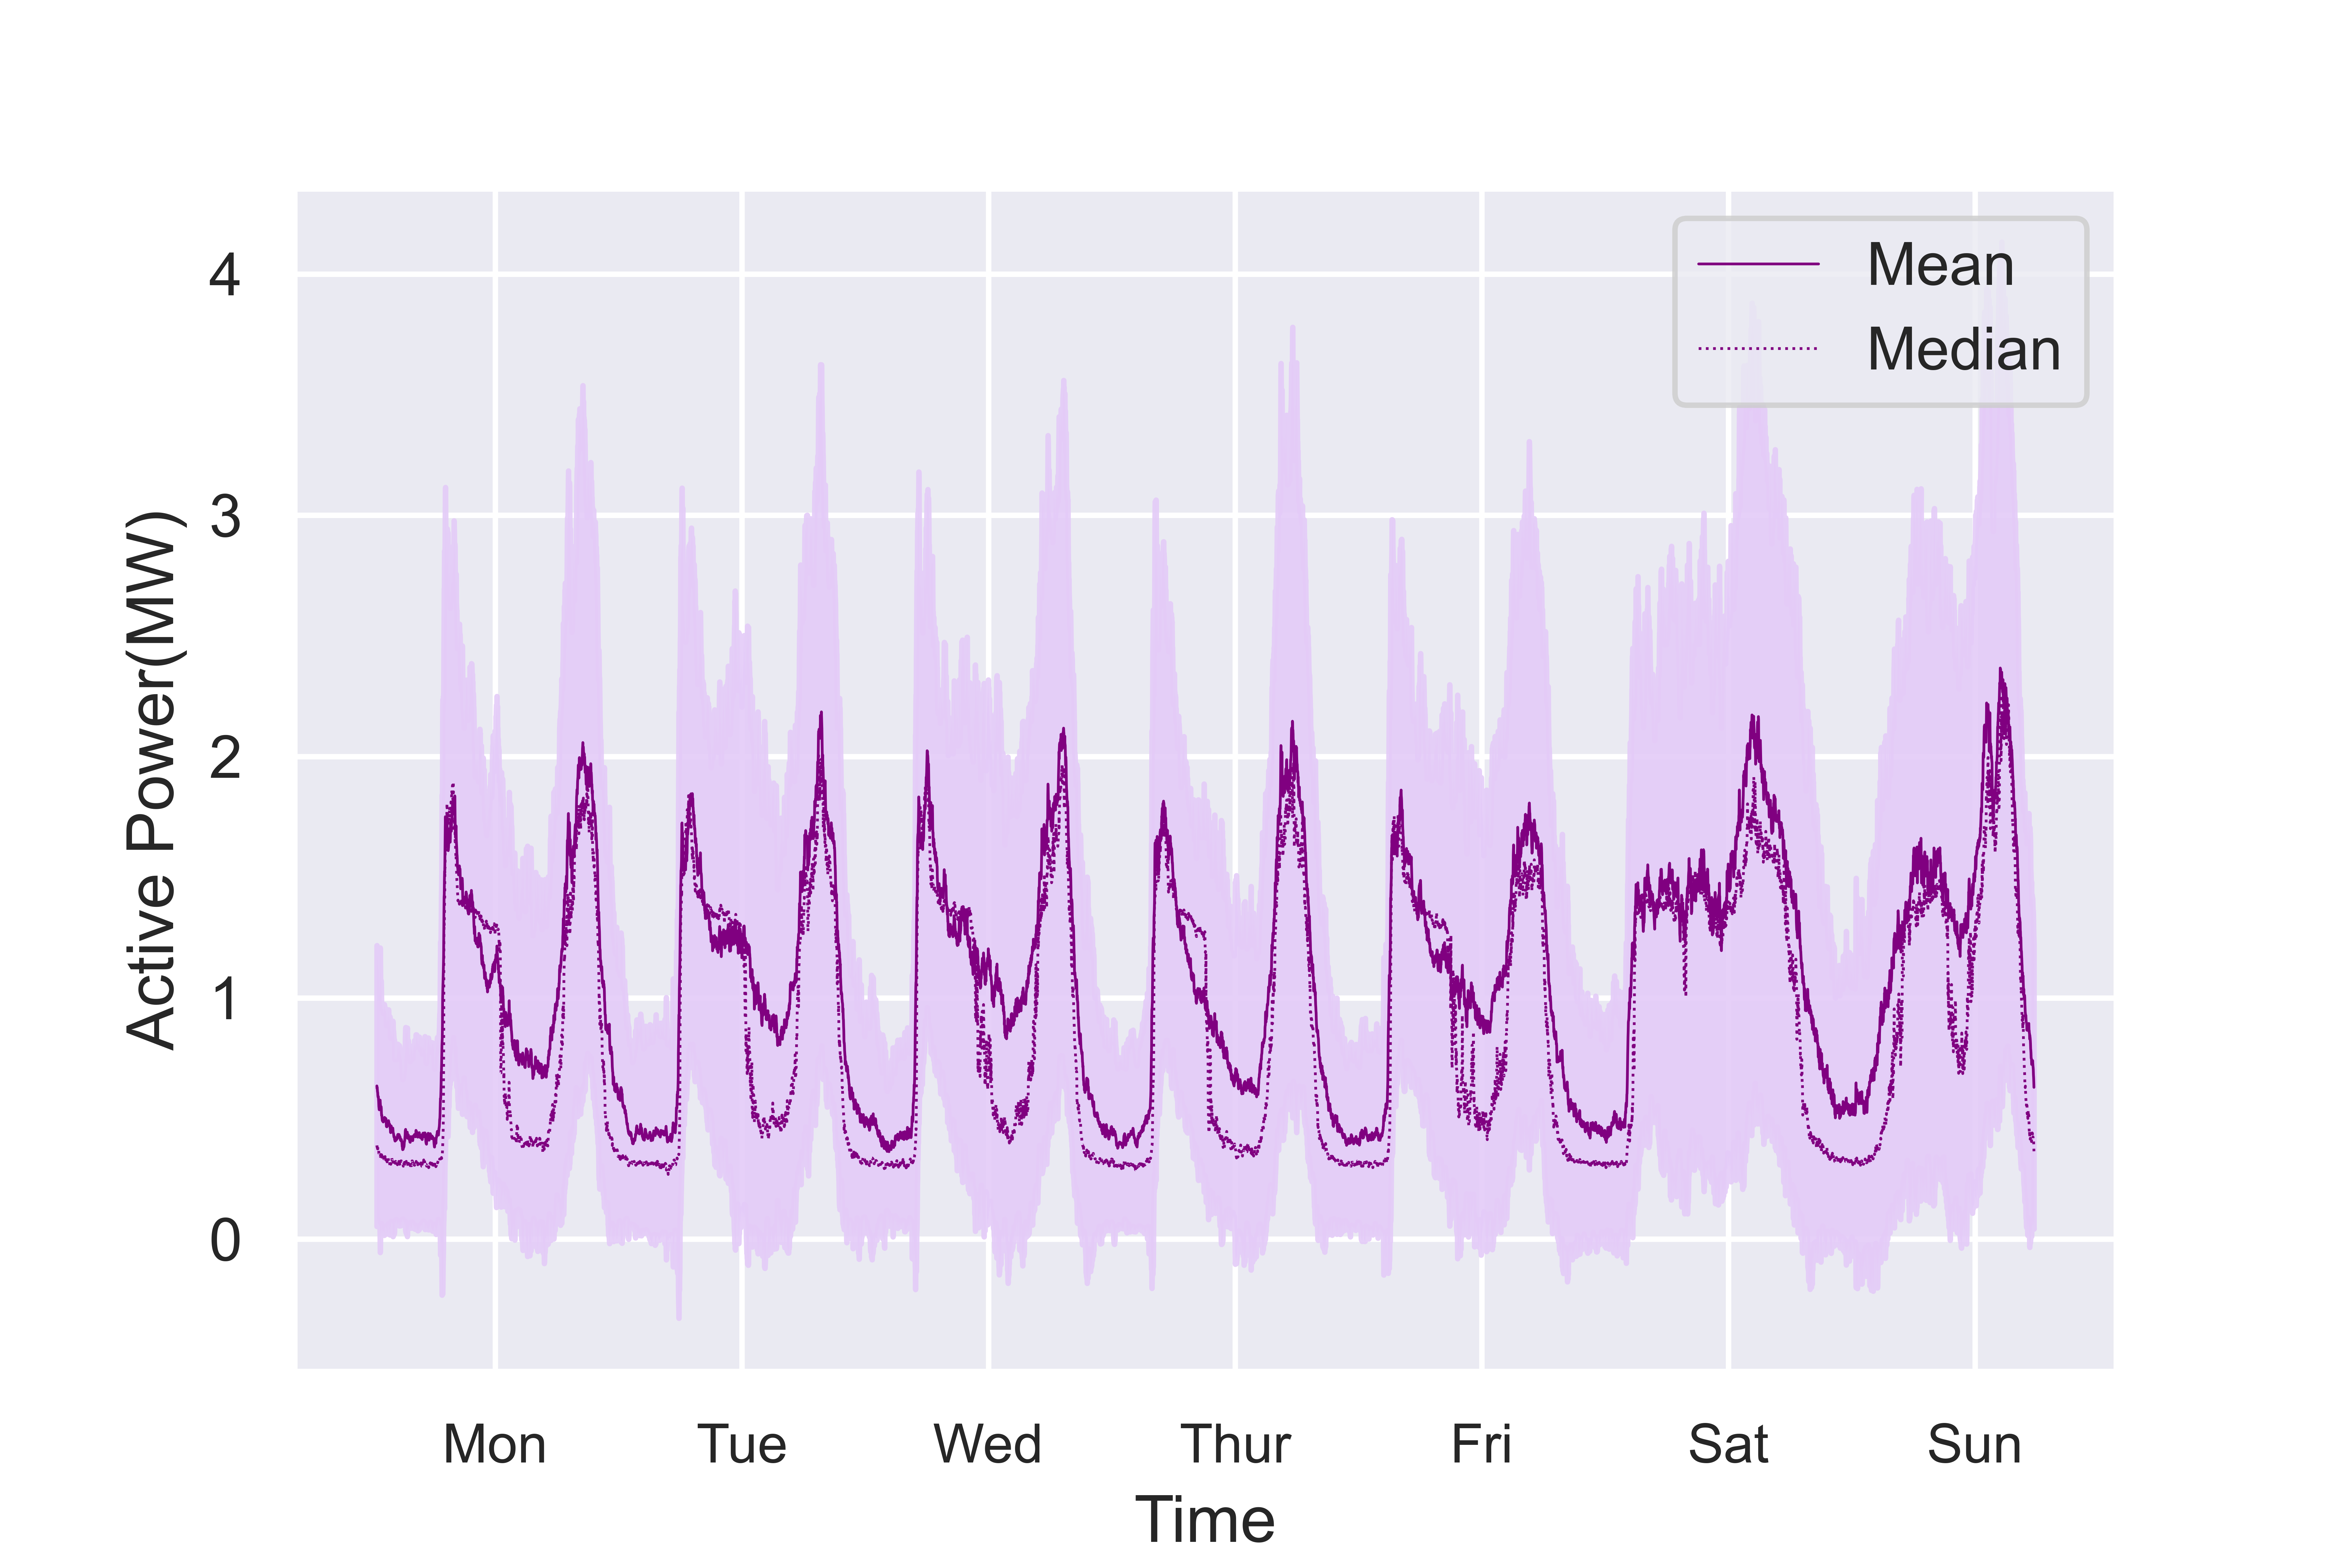
\includegraphics[width=\textwidth]{../Figures/uci.PNG}
% \end{figure}

\begin{figure}[H]
    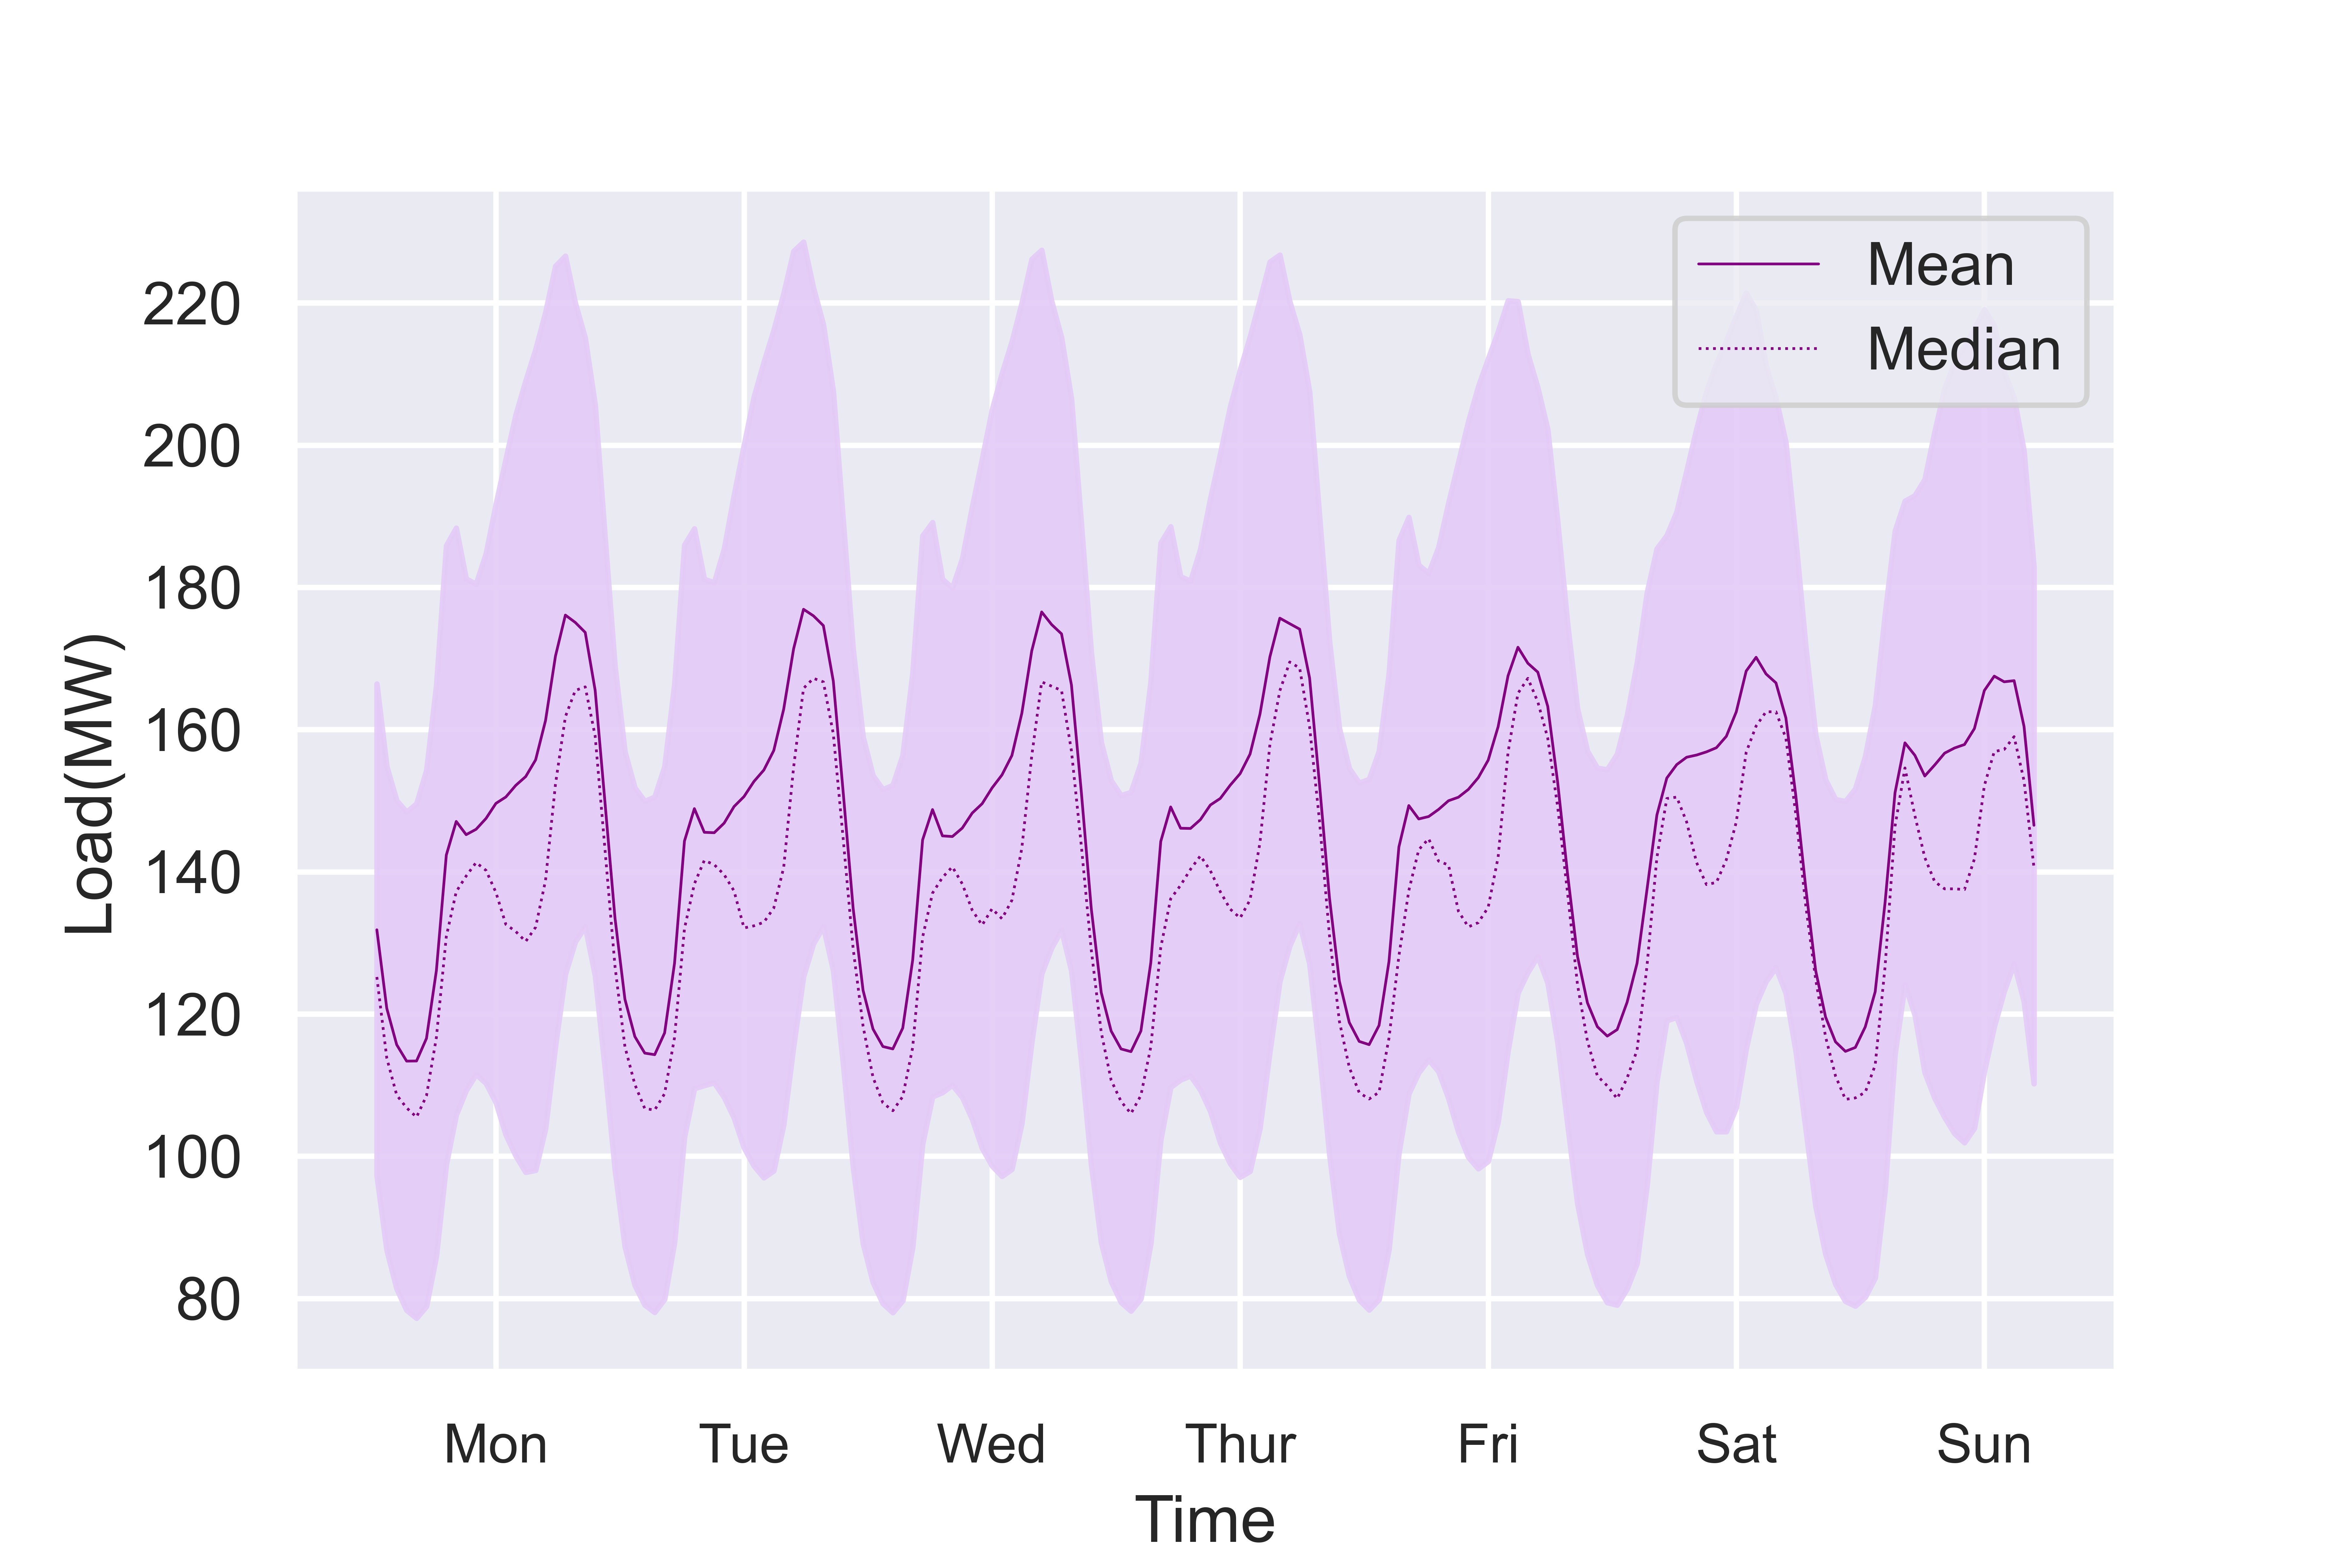
\includegraphics[width=\textwidth]{../Figures/gef2014.PNG}
    \caption{GEFCom2014 Electric Load}
    \label{fig:gefc2014}
\end{figure}

\section{Models and evaluate}
In this experiment, TCN together with FNN, RNN, GRU, seq2seq models were adopted. And we use $MSE$,$RMSE$, $MAE$ and $R^2$ to evaluate models' performance. Besides, we also try to evaluate detection accuracy by using \textit{long-short prediction difference(LSPD)}. The definitions of these metrics are noted below.

$$RMSE = \sqrt[2]{\frac{1}{N}\sum_{i=0}^{N-1}\frac{1}{n_o}\sum_{t=0}^{n_o-1}(\hat{y_i}[t]-y_i[t])^2} $$
$$MAE = \frac{1}{N}\sum_{i=0}^{N-1}\frac{1}{n_o}\sum_{t=0}^{n_o-1}|\hat{y_i}[t]-y_i[t]|$$
$$LSPD = \frac{ShortTermMSE}{SongTermMSE}$$
$$MSE = \frac{1}{N}\sum_{i=0}^{N-1}\frac{1}{n_o}\sum_{t=0}^{n_o-1}(\hat{y_i}[t]-y_i[t])^2$$


\section{Programming Environment and experiment settings}
We adopted Keras framework to help us build such a experiment, related hardware and software dependencies as following table \ref{tab:dependencies}. 

\begin{table}[H]
\centering
\begin{tabular}{l l}
\toprule
\textbf{Item} & \textbf{Dependencies}  \\
\midrule
Cloud Computation Support & Supported by CityU Burgundy HPC\\
Python & Version 3.6.x  \\
TensorFlow& Version 2.1 \\
Keras& 2.3.1 \\
sacred& 0.7.5 \\
\bottomrule
\end{tabular}
\caption{Hardware and software dependencies}
\label{tab:dependencies}
\end{table}

\section{Numeric results and discussion}

\subsection{Models' performance comparasion}
\begin{table}[H]
\centering
\begin{tabular}{l r r r r}
\toprule
\textbf{Model} & \textbf{MSE} & \textbf{MAE} & \textbf{$R^2$}& \textbf{RMSE}\\
\midrule
TCN & 772.69& 18.57& 0.54& 27.80\\
GRU\-Rec & 746.99& 19.64& 0.79& 27.33 \\
GRU\-MIMO& 423.54& 15.50& 0.82& 20.58 \\
Vanilla RNN& 2275.85& 30.47& 0.73& 47.71 \\
LSTM\-Rec & 697.94& 24.65& 0.76& 26.42 \\
LSTM\-MIMO & 378.31& 16.18& 0.84& 19.45 \\
FNN & 330.90& 10.53& \color{red}0.88& 18.19 \\
\bottomrule
\end{tabular}
\caption{Models' Performance Comparasion}
\label{tab:models}
\end{table}

From table \ref{tab:models} we can find that FNN shows the best fit result amongst all the models we have adopted, with the $R^2 = 0.88$. Since TCN did not reach a good detection performance as other models did, so we did more sub-experiments on TCN, mainly on hyper-parameters modification and different datasets (not yet).


\begin{figure}
    \centering
    \begin{subfigure}[b]{0.55\textwidth}
        \centering
        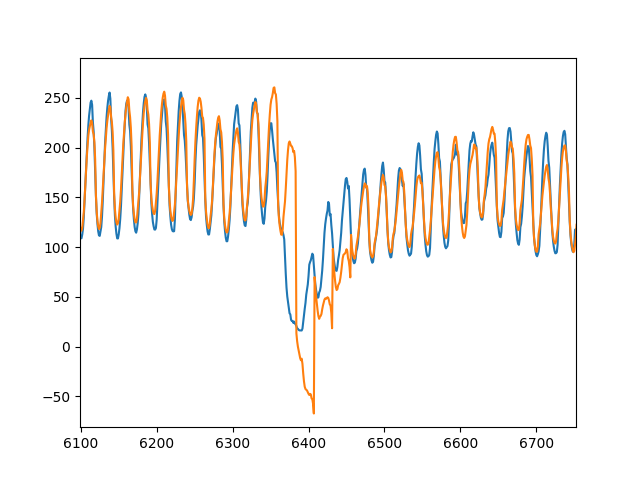
\includegraphics[width=\textwidth]{../Figures/fnn-1.png}
        \caption{fnn1}
        \label{fig:fnn1}
    \end{subfigure}
    \hfill
    \begin{subfigure}[b]{0.55\textwidth}
        \centering
        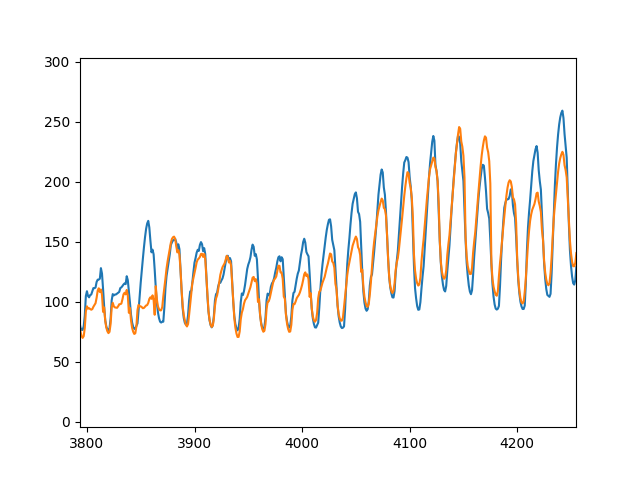
\includegraphics[width=\textwidth]{../Figures/fnn-2.png}
        \caption{fnn2}
        \label{fig:fnn2}
    \end{subfigure}
    \hfill
    \begin{subfigure}[b]{0.55\textwidth}
        \centering
        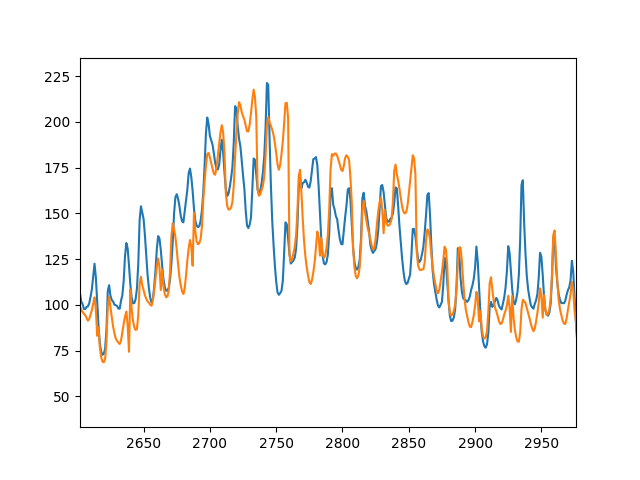
\includegraphics[width=\textwidth]{../Figures/fnn-3.png}
        \caption{fnn3}
        \label{fig:fnn3}
    \end{subfigure}
    \hfill
    \begin{subfigure}[b]{0.55\textwidth}
        \centering
        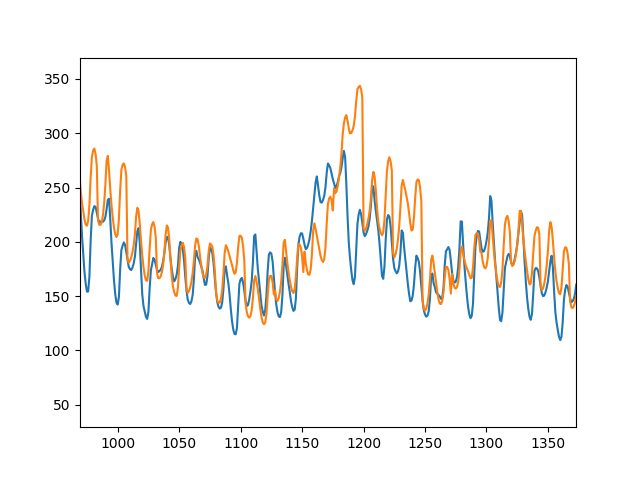
\includegraphics[width=\textwidth]{../Figures/fnn-4.png}
        \caption{fnn4}
        \label{fig:fnn4}
    \end{subfigure}
       \caption{FNN results in plot}
       \label{fig:fnn}
\end{figure}


\begin{figure}
    \centering
    \begin{subfigure}[b]{0.55\textwidth}
        \centering
        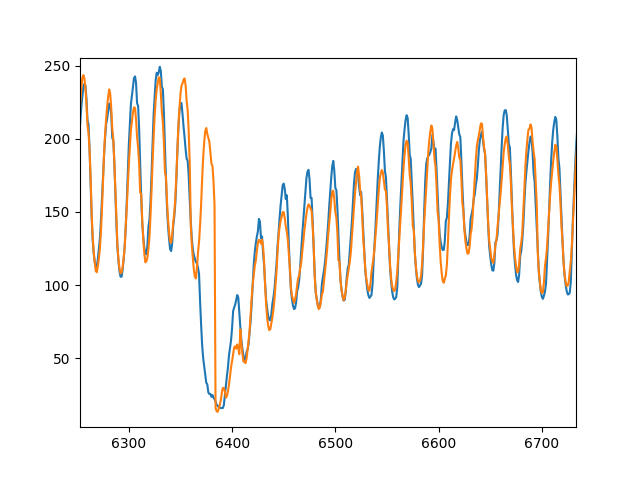
\includegraphics[width=\textwidth]{../Figures/tcn-1.png}
        \caption{tcn1}
        \label{fig:tcn1}
    \end{subfigure}
    \hfill
    \begin{subfigure}[b]{0.55\textwidth}
        \centering
        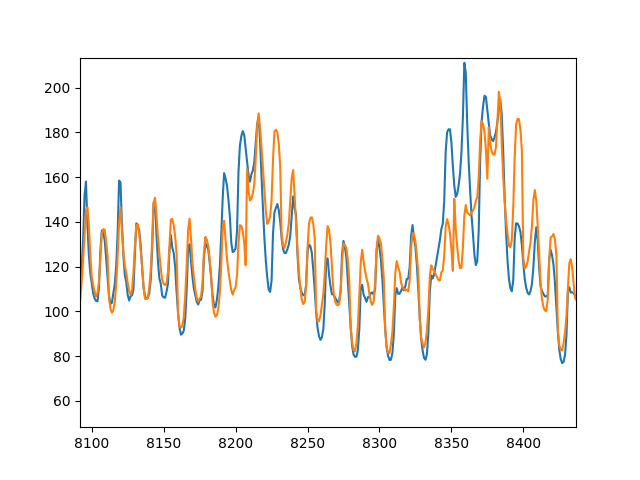
\includegraphics[width=\textwidth]{../Figures/tcn-2.png}
        \caption{tcn2}
        \label{fig:tcn2}
    \end{subfigure}
    \hfill
    \begin{subfigure}[b]{0.55\textwidth}
        \centering
        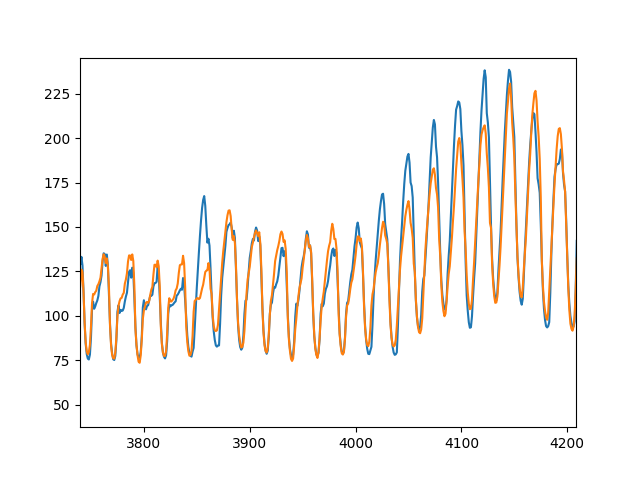
\includegraphics[width=\textwidth]{../Figures/tcn-3.png}
        \caption{tcn3}
        \label{fig:tcn3}
    \end{subfigure}
    \hfill
    \begin{subfigure}[b]{0.55\textwidth}
        \centering
        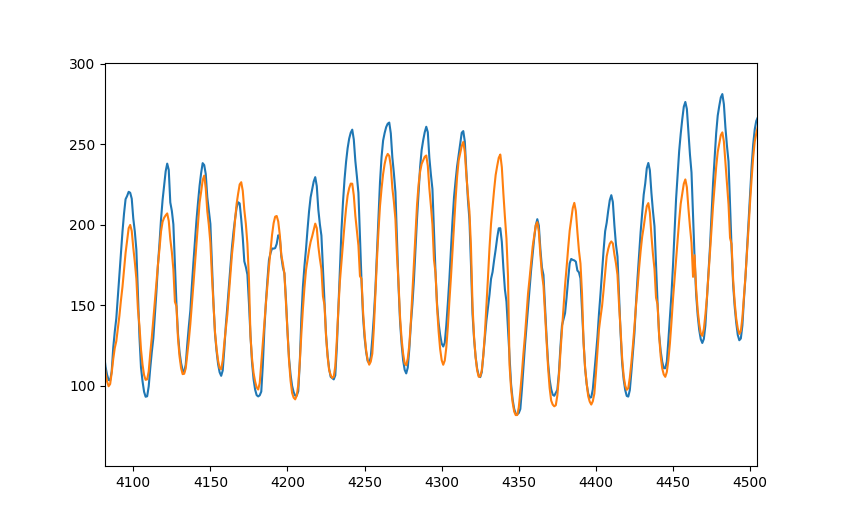
\includegraphics[width=\textwidth]{../Figures/tcn-4.png}
        \caption{tcn4}
        \label{fig:tcn4}
    \end{subfigure}
       \caption{TCN results in plot}
       \label{fig:tcn}
\end{figure}

\begin{figure}
    \centering
    \begin{subfigure}[b]{0.55\textwidth}
        \centering
        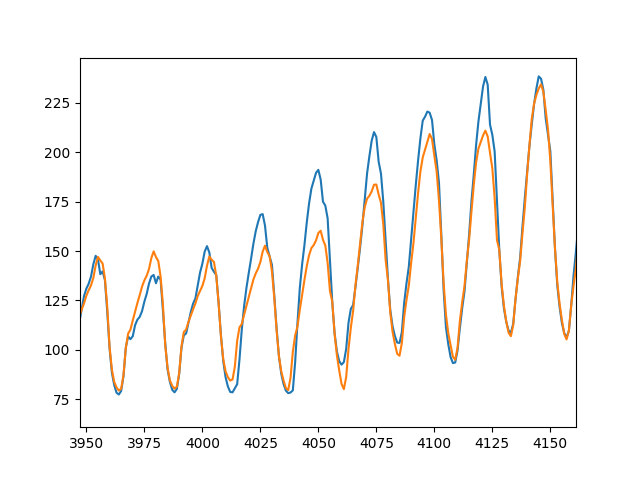
\includegraphics[width=\textwidth]{../Figures/gru-mimo-1.png}
        \caption{gru-mimo1}
        \label{fig:gru-mimo1}
    \end{subfigure}
    \hfill
    \begin{subfigure}[b]{0.55\textwidth}
        \centering
        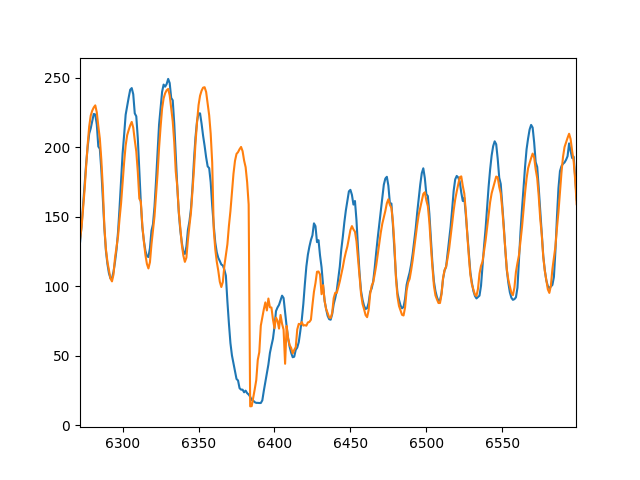
\includegraphics[width=\textwidth]{../Figures/gru-mimo-2.png}
        \caption{gru-mimo2}
        \label{fig:gru-mimo2}
    \end{subfigure}
    \hfill
    \begin{subfigure}[b]{0.55\textwidth}
        \centering
        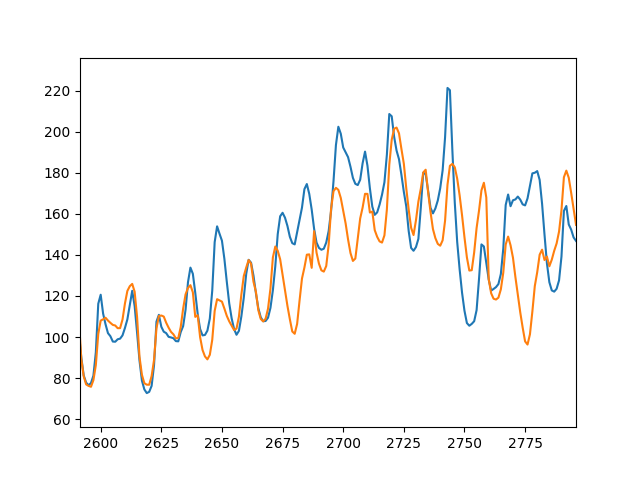
\includegraphics[width=\textwidth]{../Figures/gru-mimo-3.png}
        \caption{gru-mimo3}
        \label{fig:gru-mimo3}
    \end{subfigure}
       \caption{GRU-MIMO results in plot}
       \label{fig:gru-mimo}
\end{figure}


\subsection{TCN Improvement}
\begin{table}[H]
\centering
\begin{tabular}{l r r r r r r r r r r  r r r}
\toprule
\textbf{Test} & \textbf{Epochs} & \textbf{Input} & \textbf{Output}& \textbf{Lrate} & \textbf{L2-reg} & \textbf{OChannel} & \textbf{MSE} & \textbf{MAE} & \textbf{$R^2$}& \textbf{RMSE} \\
\midrule
Raw & 1& 96& 24& 0.001& 0.005& 32& 772.69& 18.57& 0.54& 27.80\\
T1 & \color{blue}100& 96& 24& 0.001& 0.005& 32& 280.32& 10.38& 0.84& 16.74 \\
T2 & \color{blue}30& 24& 24& 0.001& 0.005& 32& 315.89& 10.83& 0.82& 17.77 \\
T3 & 30& 48& 24& 0.001& 0.005& 32& 300.18& 10.58& 0.83& 17.33 \\
T4 & 30& 96& 24& 0.001& 0.005& 32& 280.32& 10.38& 0.84& 16.74 \\
T5 & 30& \color{blue}168& 24& 0.001& 0.005& 32& 300.18& 10.58& 0.83& 17.33 \\
T6 & 30& 336& 24& 0.001& 0.005& 32& 259.50& 9.91& 0.84& 16.11 \\ %14
T7 & 30& 336& \color{blue}48& 0.001& 0.005& 32& 370.97& 11.80& 0.76& 19.26 \\
T8 & 30& 168& 24& \color{blue}0.01& 0.005& 32& 265.36& 10.03& 0.84& 16.29 \\
T9 & 30& 168& 24& 0.001& \color{blue}0.001& 32& 256.22& 9.81& 0.86& 16.01 \\
T10 & 30& 168& 24& 0.001& \color{blue}0.01& 32& 266.83& 9.81& 0.84& 16.34 \\
T11 & 30& 168& 24& 0.001& 0.01& \color{blue}16& 254.09& 9.61& \color{red}0.864& 15.94 \\
\bottomrule
\end{tabular}
\caption{Hyper Parameters Comparasion}
\label{tab:hyper}
\end{table}

As table \ref{tab:hyper} showed, we try to change input length and output length , which are how many hours will be used as a sliding window's input and output, to make the model more sensibale, and according to test metrics, we found that TCN will give the best performance when we try to use 7 days(168 hours)' electricity load to predict one day(24 hours)'s electricity load, we got $R^2 \geq 0.85$.

As for Epochs, which means the number of passes of the entire training dataset the deep learning algorithm has completed, significantly influenced TCN's training, and 30 epochs will give the most economical training results. We guess this is because TCN needs more passes to fit a good state, for it lacks some mechanism like LSTM's recurrent units.

Learning rate, L2-regulation, and the number of out channels were also influenced, but they mainly contributed to improving computation speed.


